\subsection{Acoustic characteristics of the vowel and consonants}

Below is an account of the spectral behaviour of the word. I have moved most of the discussion of formant frequencies below this figure and slightly lower down (section \ref{x:formants}). The first figure is taken from Praat from 0-10kHz with a window length of 0.015.

\begin{figure}[H] 
	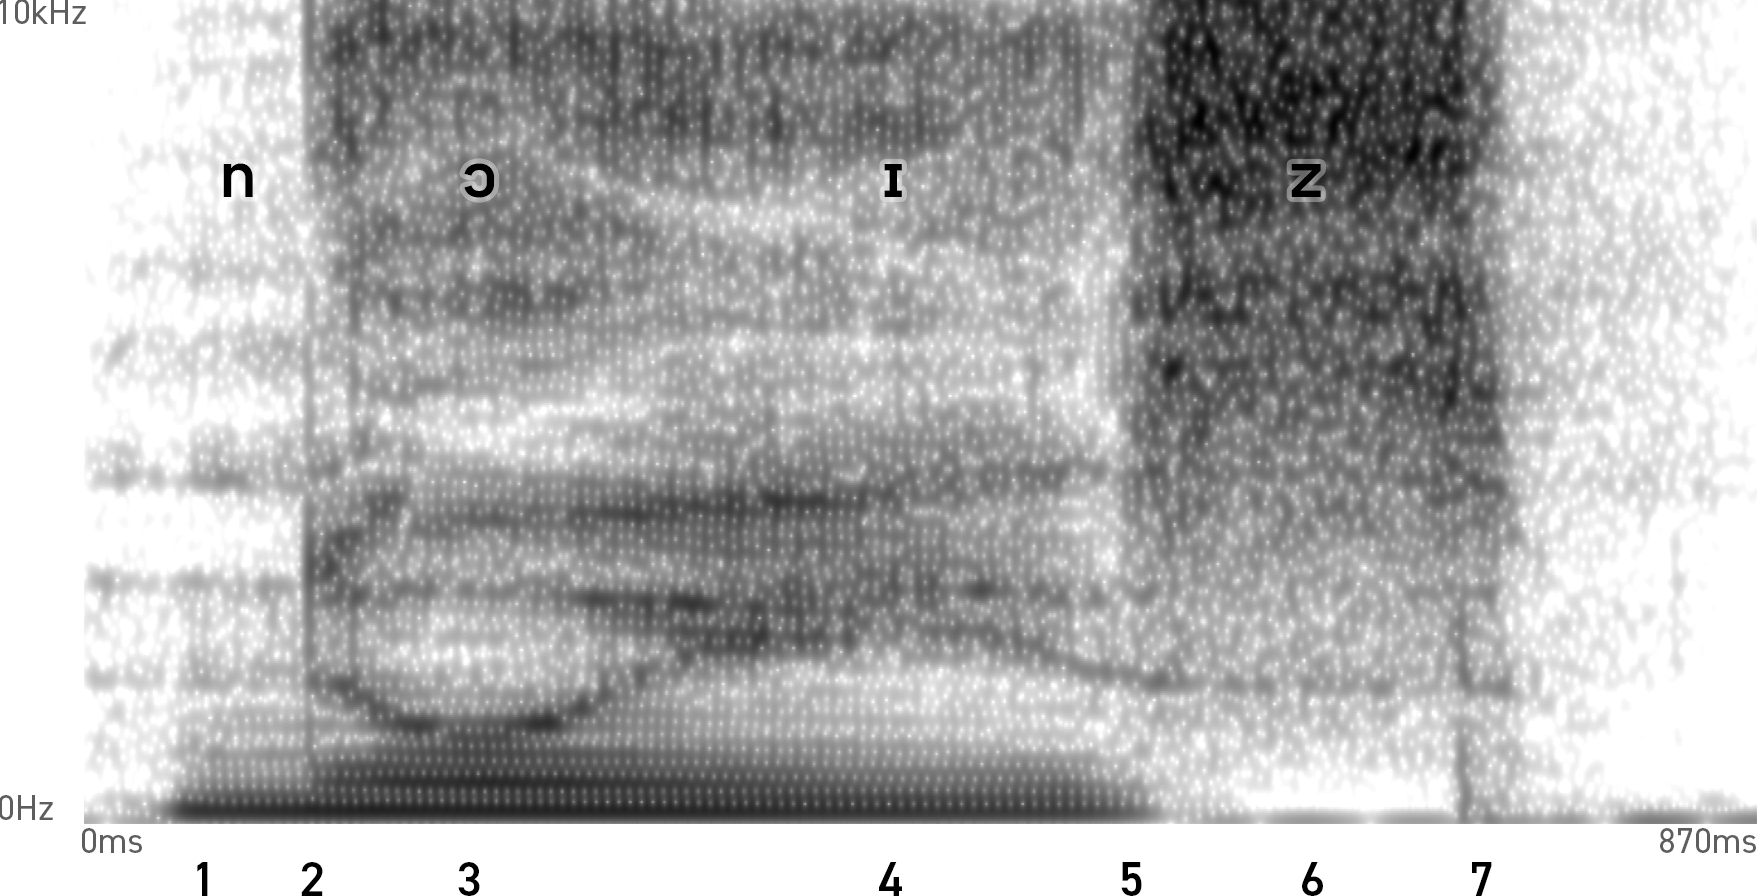
\includegraphics[width=1\textwidth]{acoustics.png}
\end{figure}

\begin{enumerate}
	\item Onset of \ipa{n}, 69ms. Strong fundamental relative to harmonics, formants are present but not prominent. Intensity increasing gradually until 2.
	\item Rapid change to vowel, about 12ms during which time the peak amplitude increases and there are much more prominent higher frequency noise and harmonics. The formants are more prominent and characteristic of \ipa{ʌ}.
	\item Over the course of about 85ms the vowel transitions to \ipa{ɔ}. $F_2$ lowers distinctly to 1kHz. $F_1$ lifts slightly to meet it. The prominence of the fundamental increases relative to the harmonics.
	\item Transition to \ipa{i} over 200ms. $F_2$ raises to 2300Hz. $F_1$ lowers slightly. The prominence of the fundamental decreases but only slightly.
	\item For another 100ms $F_2$ drops slightly and then there's a small window of about 30ms where the level of the harmonics drops sharply (the spectral tilt is much more weighted towards the fundamental) and the level of the fundamental starts decreasing. Then noise is introduced as the \ipa{z} begins.
	\item The noise is well represented up to about 17kHz before it starts to drop off (not shown above). The distribution is indicated in Figure \ref{fig:z_slice}, page \pageref{fig:z_slice}, with spectral peaks at 9300kHz and 8500kHz, although this is not constant. The noise lasts for 160ms. For the first 40ms the fundamental is still prominent but it begins to drop off and the sound is more characteristic of \ipa{s}.
	\item Noise decays relatively uniformly over 33ms as the word ends.
\end{enumerate}

\subsubsection{Formants} \label{x:formants}

%
\begin{figure}[H] 
	\centering
	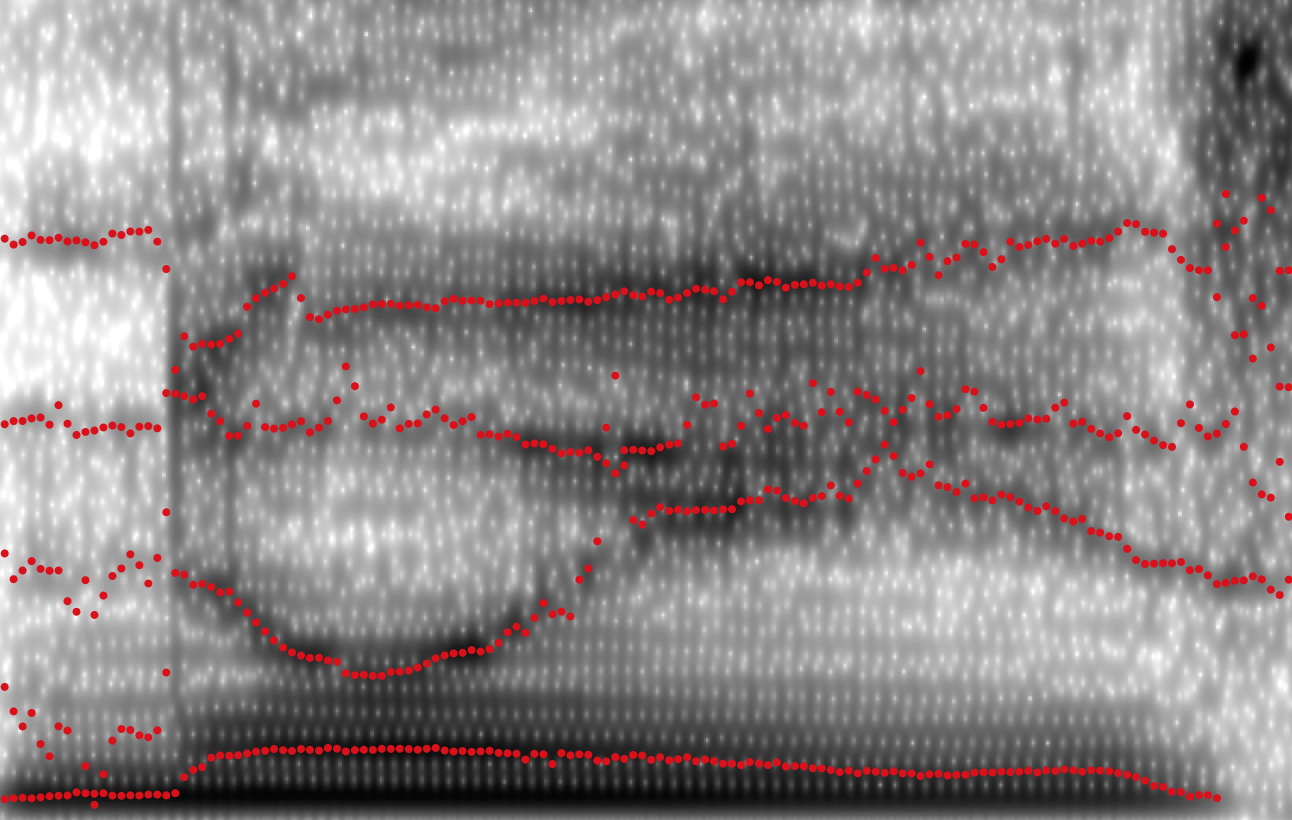
\includegraphics[width=0.7\textwidth]{formants.png}
	\caption{Movement of the first four formants according to Praat. Max formant limited to 4800Hz, window length 0.015. Spectrogram 0-6kHz, window length 0.01, dynamic range 70dB.}
	\label{fig:formants}
\end{figure}
%
\renewcommand{\arraystretch}{0.9}
\begin{center}
	\csvautotabular{formants.csv}
\end{center}
\renewcommand{\arraystretch}{1.3}
